Considerando, ora, la stessa architettura software precedentemente esposta, si potrebbe fare un ragionamento riguardo il periodo di clock considerato. In particolare, si potrebbe pensare di utilizzare un periodo minore per analizzare come il tool gestisce la situazione associata. L'idea è quella di diminuire tale periodo senza andare oltre un margine. Questo vuol dire considerare lo slack associato alla soluzione iniziale e ridurlo fin quando è possibile, cioè fin quando i constraint di timing non sono violati. Ciò che dovremmo aspettarci è che il tool riesca a gestire la stessa architettura con un periodo di clock minore, rispetto a quello della soluzione iniziale non ottimizzata, garantendo in alcuni casi delle ottimizzazioni effettuate dallo stesso tool. L'ideale sarebbe ottenere una soluzione che mi permette di avere un giusto trade-off tra latenza (intesa come cicli di clock per ottenere un risultato), potenza e risorse utilizzate.
\\
Qui di seguito verranno presentati i report associati alla sintesi, C/RTL Cosimulation ed Export RTL considerando un range di periodo di clock pari a $[10ns, 3ns]$. In particolare, le soluzioni analizzate non sono state considerate con un periodo del clock minore a 3ns dato che, come verrà mostrato e analizzato successivamente, in corrispondenza di un periodo del clock pari a 3ns, la soluzione hardware implementata all'interno di Vivado presenta un WNS negativo comportando, di conseguenza, la violazione dei constraint di timing.
\begin{table}[H]
    \centering
    \begin{minipage}[t]{0.38\linewidth}
        \centering
        \begin{tabular}{|c|c|c|c|c|}
            \hline
            \textbf{Solution} & \textbf{Clock} & \textbf{Target} & \textbf{Estimated} & \textbf{Uncertainty} \\
            \hline
            clk=10ns & ap\_clk & 10.00 & 8.510 & 1.25 \\
            \hline
            clk=9ns & ap\_clk & 9.00 & 6.912 & 1.12 \\
            \hline
            clk=8ns & ap\_clk & 8.00 & 6.912 & 1 \\
            \hline
            clk=7ns & ap\_clk & 7.00 & 5.745 & 0.88 \\
            \hline
            clk=6ns & ap\_clk & 6.00 & 4.644 & 0.75 \\
            \hline
            clk=5ns & ap\_clk & 5.00 & 4.321 & 0.62 \\
            \hline
            clk=4ns & ap\_clk & 4.00 & 3.254 & 0.5 \\
            \hline
            clk=3ns & ap\_clk & 3.00 & 2.552 & 0.38 \\
            \hline
        \end{tabular}
        \caption{HLS Operation Chaining Solution Timing Summary (ns)}
        \label{tab:hls-operation-chaining-solution-timing-summary}
    \end{minipage}
    \hfill
    \begin{minipage}[t]{0.38\linewidth}
        \centering
        \begin{tabular}{|c|c|c|c|c|}
            \hline
            \multicolumn{1}{|c|}{\textbf{Solution}} & \multicolumn{2}{|c|}{\textbf{Latency}} & \multicolumn{2}{|c|}{\textbf{Interval}} \\
            & min & max & min & max \\
            \hline
            clk=10ns & 23 & 45 & 23 & 45 \\
            \hline
            clk=9ns & 24 & 57 & 24 & 57 \\
            \hline
            clk=8ns & 24 & 57 & 24 & 57 \\
            \hline
            clk=7ns & 25 & 69 & 25 & 69 \\
            \hline
            clk=6ns & 27 & 93 & 27 & 93 \\
            \hline
            clk=5ns & 27 & 93 & 27 & 93 \\
            \hline
            clk=4ns & 40 & 139 & 40 & 139 \\
            \hline
            clk=3ns & 40 & 139 & 40 & 139 \\
            \hline
        \end{tabular}
        \caption{HLS Operation Chaining Solution Latency Summary (clock cycles)}
        \label{tab:hls-unoptimized-solution-latency-summary}
    \end{minipage}
\end{table}

\begin{table}[H]
    \centering
    \begin{tabular}{|c|c|c|c|c|c|c|c|c|}
        \hline
        \multicolumn{1}{|c|}{\textbf{Solution}} & \multicolumn{1}{|c|}{Loop} & \multicolumn{2}{|c|}{\textbf{Latency}} & \multicolumn{1}{c|}{\textbf{Iteration Latency}} & \multicolumn{2}{c|}{\textbf{Initiation Interval}} & \multicolumn{1}{c|}{\textbf{Trip Count}}  \\
        & Name & min & max &  & achieved & target &  \\
        \hline
        clk=10ns & - loop & 22 & 44 & 2 $\sim$ 4 & - & - & 11 \\
        \hline
        clk=9ns & - loop & 22 & 55 & 2 $\sim$ 5 & - & - & 11 \\
        \hline
        clk=8ns & - loop & 22 & 55 & 2 $\sim$ 5 & - & - & 11 \\
        \hline
        clk=7ns & - loop & 22 & 66 & 2 $\sim$ 6 & - & - & 11 \\
        \hline
        clk=6ns & - loop & 22 & 88 & 2 $\sim$ 8 & - & - & 11 \\
        \hline
        clk=5ns & - loop & 22 & 88 & 2 $\sim$ 8 & - & - & 11 \\
        \hline
        clk=4ns & - loop & 33 & 132 & 3 $\sim$ 12 & - & - & 11 \\
        \hline
        clk=3ns & - loop & 33 & 132 & 3 $\sim$ 12 & - & - & 11 \\
        \hline
    \end{tabular}
    \caption{HLS Operation Chaining Solution Latency Loops Summary }
    \label{tab:hls-operation-chaining-solution-loop-summary}
\end{table}
Si può notare come al diminuire del periodo di clock, la latenza totale e la latenza per ogni iterazione aumentano rispettivamente. Questo è dovuto al fatto che, considerando un periodo di clock sempre minore, il tool cerca di garantire il minor tempo di latenza affinché le operazioni presenti all'interno del loop vengano eseguite correttamente. Pertanto, se il periodo del clock diminuisce, questo si traduce in un aumento dei cicli di clock richiesti per ogni iterazione. Bisogna notare che, in corrispondenza di alcune soluzioni, alcuni parametri assumono valori uguali. In particolare, tale situazione si verifica in corrispondenza delle soluzioni aventi periodo del clock pari a 9ns e 8ns e anche in corrispondenza di 6ns e 5ns e, infine, 4ns e 3ns. Questa peculiarità potrebbe essere sfruttata successivamente, considerando ulteriori design parameters di confronto, per la scelta di un trade-off opportuno. Dal momento che il tool cerca di garantire il soddisfacimento di tali operazioni complesse con un minore periodo di clock, quello che ci si aspetta è una utilizzazione delle risorse stimate e, in particolare, un aumento di quest'ultime al diminuire del periodo di clock.
\begin{table}[H]
    \centering
    \begin{tabular}{|c|c|c|c|c|}
        \hline
        \textbf{Solution} & \textbf{BRAM} & \textbf{DSP} & \textbf{FF} & \textbf{LUT} \\
        \hline
        clk=10ns & 0 & 4 & 287 & 233 \\
        \hline
        clk=9ns & 0 & 4 & 619 & 301 \\
        \hline
        clk=8ns & 0 & 4 & 619 & 301 \\
        \hline
        clk=7ns & 0 & 4 & 623 & 305 \\
        \hline
        clk=6ns & 0 & 4 & 725 & 221 \\
        \hline
        clk=5ns & 0 & 4 & 725 & 221 \\
        \hline
        clk=4ns & 0 & 4 & 832 & 286 \\
        \hline
        clk=3ns & 0 & 4 & 832 & 286 \\
        \hline
    \end{tabular}
    \caption{HLS Operation Chaining Solution Utilization Estimates [\#]}
    \label{tab:vivado-operation-chaining-solution-utilization-report}
\end{table}
Si evidenzia quanto citato precedentemente e, inoltre, si può notare come, anche in questo caso, in corrispondenza di alcune soluzioni hardware, l'utilizzazione delle risorse risulta essere la medesima. In particolare, è possibile già effettuare una riflessione riguardo i risultati ottenuti dopo il processo di sintesi. Si può notare come, in corrispondenza delle soluzioni hardware con clk=9ns e clk=8ns si ha lo stessa latency, iteration latency e utilizzazione delle risorse. Ma soprattutto, facendo riferimento alla soluzione con periodo di clock pari a 7ns, la latency e l'iteration latency aumentano di un fattore pari a 11 (rispetto alle altre soluzioni dove i valori sono di gran lunga maggiori) e l'utilizzazione di FF e LUT (dal momento che il numero di BRAM e DSP utilizzati è il medesimo) risulta essere aumentata rispettivamente del 0.6\% e del 1.32\%. Pertanto, a fronte del processo di sintesi, la soluzione hardware avente periodo di clock pari a 7ns si potrebbe già considerare come candidata al trade-off sopra citato.

\begin{table}[H]
    \centering
    \begin{tabular}{|c|c|c|c|c|c|c|c|c|}
        \hline
        \multicolumn{1}{|c|}{\textbf{Solution}} & \multicolumn{1}{|c|}{RTL} & \multicolumn{1}{|c|}{Status} & \multicolumn{3}{c|}{\textbf{Latency}} & \multicolumn{3}{c|}{\textbf{Interval}} \\
        & &  & min & avg & max & min & avg & max \\
        \hline
        clk=10ns & VHDL & Pass & 43 & 43 & 44 & 43 & 43 & 44 \\
        \hline
        clk=9ns & VHDL & Pass & 54 & 54 & 55 & 54 & 54 & 55 \\
        \hline
        clk=8ns & VHDL & Pass & 54 & 54 & 55 & 54 & 54 & 55 \\
        \hline
        clk=7ns & VHDL & Pass & 65 & 65 & 66 & 65 & 65 & 66 \\
        \hline
        clk=6ns & VHDL & Pass & 87 & 87 & 88 & 87 & 87 & 88 \\
        \hline
        clk=5ns & VHDL & Pass & 87 & 87 & 88 & 87 & 87 & 88 \\
        \hline
        clk=4ns & VHDL & Pass & 130 & 130 & 131 & 130 & 130 & 131 \\
        \hline
        clk=4ns & VHDL & Pass & 130 & 130 & 131 & 130 & 130 & 131 \\
        \hline
        clk=3ns & VHDL & Pass & 130 & 130 & 131 & 130 & 130 & 131 \\
        \hline
    \end{tabular}
    \caption{HLS Operation Chaining Solution C/RTL Cosimulation Report }
    \label{tab:hls-operation-chaining-solution-cosimulation-report}
\end{table}

\begin{table}[H]
    \centering
    \begin{tabular}{|c|c|c|c|c|c|c|c|c|}
        \hline
        \textbf{Solution} & \textbf{SLICE} & \textbf{LUT} & \textbf{FF} & \textbf{DSP} & \textbf{BRAM} & \textbf{CP} & \textbf{CP} & \textbf{CP} \\
        & & & & & & \textbf{required} & \textbf{achieved} & \textbf{achieved}\\
        & & & & & & & \textbf{post-} & \textbf{post-}\\
        & & & & & & & \textbf{synthesis} & \textbf{implementation}\\
        \hline
        clk=10ns & 81 & 275 & 160 & 2 & 0 & 10 & 5.745 & 6.41 \\
        \hline
        clk=9ns & 88 & 276 & 226 & 2 & 0 & 9 & 5.745 & 6.059 \\
        \hline
        clk=8ns & 89 & 276 & 226 & 2 & 0 & 8 & 5.745 & 6.034 \\
        \hline
        clk=7ns & 75 & 186 & 222 & 2 & 0 & 7 & 5.745 & 5.692 \\
        \hline
        clk=6ns & 76 & 186 & 241 & 2 & 0 & 6 & 4.823 & 4.364 \\
        \hline
        clk=5ns & 96 & 186 & 258 & 2 & 0 & 5 & 4.823 & 4.282 \\
        \hline
        clk=4ns & 114 & 188 & 376 & 2 & 0 & 4 & 3.667 & 3.724 \\
        \hline
        clk=3ns & 107 & 192 & 377 & 4 & 0 & 3 & 3.667 & 3.627 \\
        \hline
    \end{tabular}
    \caption{HLS Operation Chaining Solution Export RTL Report}
    \label{tab:vivado-operation-chaining-solution-export-rtl-report}
\end{table}

Si può notare come la soluzione ottimale precedentemente proposta risulta essere la migliore tra quelle citate. Infatti, è possibile evidenziare che rispetto alle altre soluzioni presenta il minor numero di risorse stimate dopo aver effettuato l'Export RTL in HLS. 
\\
Pertanto, si può affermare che il tool, in corrispondenza di un periodo di clock pari a 7ns, è riuscito ad effettuare delle ottimizzazioni che hanno permesso di ottenere un minimo aumento della latenza e una diminuzione delle risorse utilizzate.
\\
Quindi, considerando constraint di clock differenti per ogni IP importato in Vivado, si procede con la sintesi, l'implementazione, la Post-Implementation Timing Simulation e la generazione del file .saif per ogni soluzione corrispondente.
\lstinputlisting[language=VHDL]{solutions/operation_chaining/10ns/clk_constraint.xdc}
\lstinputlisting[language=VHDL]{solutions/operation_chaining/9ns/clk_constraint.xdc}
\lstinputlisting[language=VHDL]{solutions/operation_chaining/8ns/clk_constraint.xdc}
\lstinputlisting[language=VHDL]{solutions/operation_chaining/7ns/clk_constraint.xdc}
\lstinputlisting[language=VHDL]{solutions/operation_chaining/6ns/clk_constraint.xdc}
\lstinputlisting[language=VHDL]{solutions/operation_chaining/5ns/clk_constraint.xdc}
\lstinputlisting[language=VHDL]{solutions/operation_chaining/4ns/clk_constraint.xdc}
\lstinputlisting[language=VHDL]{solutions/operation_chaining/3ns/clk_constraint.xdc}

In particolare, qui di seguito verranno mostrati e analizzati soltanto i report corrispondenti alle soluzioni avente periodo di clock compreso nell'intervallo $[10ns,4ns]$. Infatti, è possibile notare come, in corrrispondenza del periodo di clock pari a 3ns, i constraint di timing siano violati.
\begin{figure}[H]
    \centering
    
\includegraphics[width=\textwidth]{solutions/operation_chaining/3ns/timingrequirement.png}
    \label{fig:left}
\end{figure}
\begin{figure}[H]
    \centering
    \begin{minipage}[t]{0.45\textwidth}
        \centering
        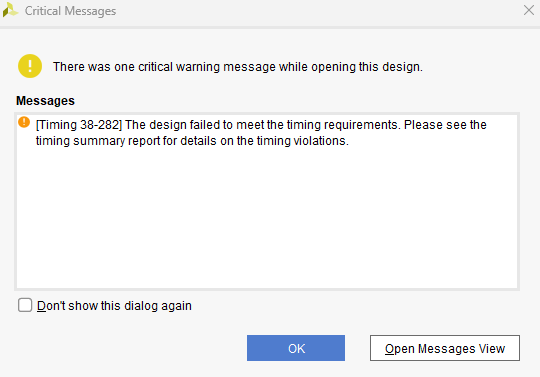
\includegraphics[width=\textwidth]{solutions/operation_chaining/3ns/critical.png}
    \caption{Vivado Operation Chaining Solution clk=3ns Timing Constraint Violated}
        \label{fig:left}
    \end{minipage}
    \hfill
    \begin{minipage}[t]{0.45\textwidth}
        \centering
        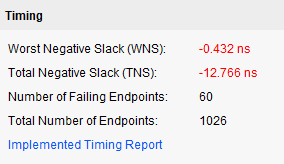
\includegraphics[width=\textwidth]{solutions/operation_chaining/3ns/wns.png}
    \caption{Vivado Operation Chaining Solution clk=3ns Timing Constraint Violated}
        \label{fig:right}
    \end{minipage}
\end{figure}

Pertanto, si procede con l'analisi dei report delle soluzioni hardware implementate in Vivado aventi periodo di clock coompreso nell'intervallo $[10ns,4ns]$.

\begin{table}[H]
    \centering
    \begin{tabular}{|c|c|c|c|c|c|c|c|}
        \hline
        \textbf{Solution} & \textbf{LUT} & \textbf{LUTRAM} & \textbf{FF} & \textbf{BRAM} & \textbf{DSP} & \textbf{IO} & \textbf{BUFG} \\
        \hline
        clk=10ns & 275 & 32 & 160 & 0 & 2 & 71 & 1 \\
        \hline
        clk=9ns & 276 & 32 & 226 & 0 & 2 & 71 & 1 \\
        \hline
        clk=8ns & 276 & 32 & 226 & 0 & 2 & 71 & 1 \\
        \hline
        clk=7ns & 186 & 32 & 222 & 0 & 4 & 71 & 1 \\
        \hline
        clk=6ns & 186 & 32 & 241 & 0 & 4 & 71 & 1 \\
        \hline
        clk=5ns & 186 & 32 & 258 & 0 & 4 & 71 & 1 \\
        \hline
        clk=4ns & 188 & 32 & 376 & 0 & 4 & 71 & 1 \\
        \hline
    \end{tabular}
    \caption{Vivado Operation Chaining Solution Utilization Report [\#]}
    \label{tab:vivado-operation-chaining-utilization-report}
\end{table}

\begin{figure}[H]
    \centering
    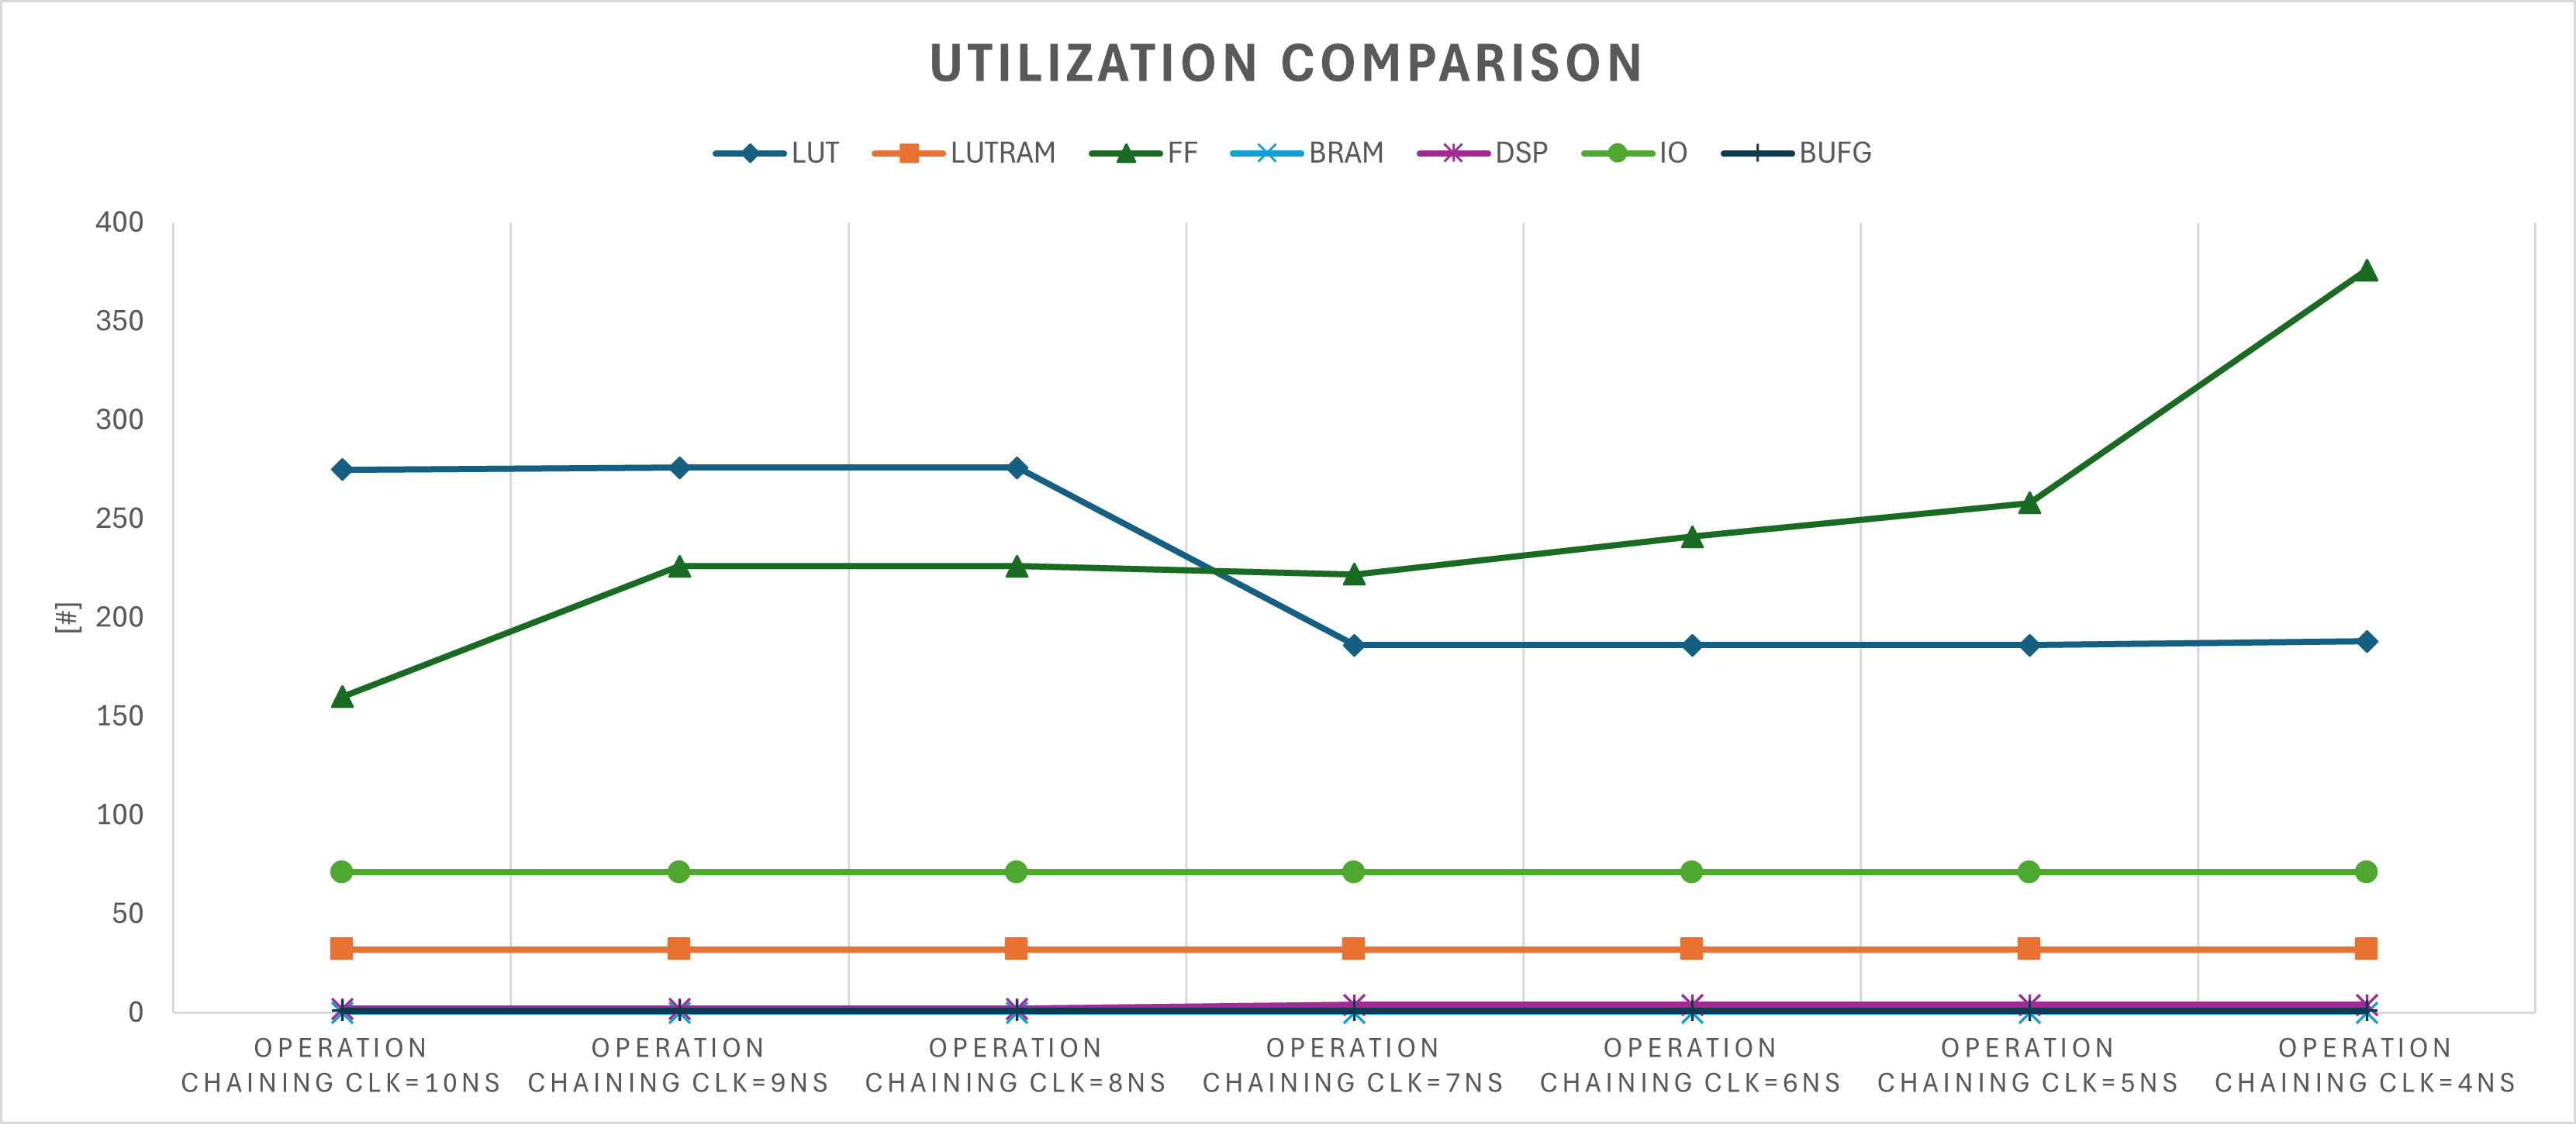
\includegraphics[width=\textwidth]{solutions/operation_chaining/operationchainingutilization.png}
    \caption{Vivado Operation Chaining Utilization Plot}
    \label{fig:vivado-operation-chaining-utilization-plot}
\end{figure}

\begin{table}[H]
    \centering
    \begin{tabular}{|c|c|c|c|c|}
        \hline
        \textbf{Solution} & \textbf{Cycles} [\#] & \textbf{Clock Constraint} [ns] & \textbf{WNS} [ns] & \textbf{Maximum Clock Frequency} [Mhz] \\
        \hline
        clk=10ns & 44 & 10 & 3.654 & 157.5795777 \\
        \hline
        clk=9ns & 55 & 9 & 3.06 & 168.3501684 \\
        \hline
        clk=8ns & 55 & 8 & 2.277 & 174.7335314 \\
        \hline
        clk=7ns & 66 & 7 & 1.33 & 176.366843 \\
        \hline
        clk=6ns & 88 & 6 & 1.573 & 225.8866049 \\
        \hline
        clk=5ns & 88 & 5 & 0.374 & 216.1694769 \\
        \hline
        clk=4ns & 131 & 4 & 0.454 & 282.0078962 \\
        \hline
    \end{tabular}
    \caption{Vivado Operation Chaining Solution Timing Report}
    \label{tab:vivado-operation-chaining-solution-timing-report}
\end{table}

\begin{figure}[H]
    \centering
    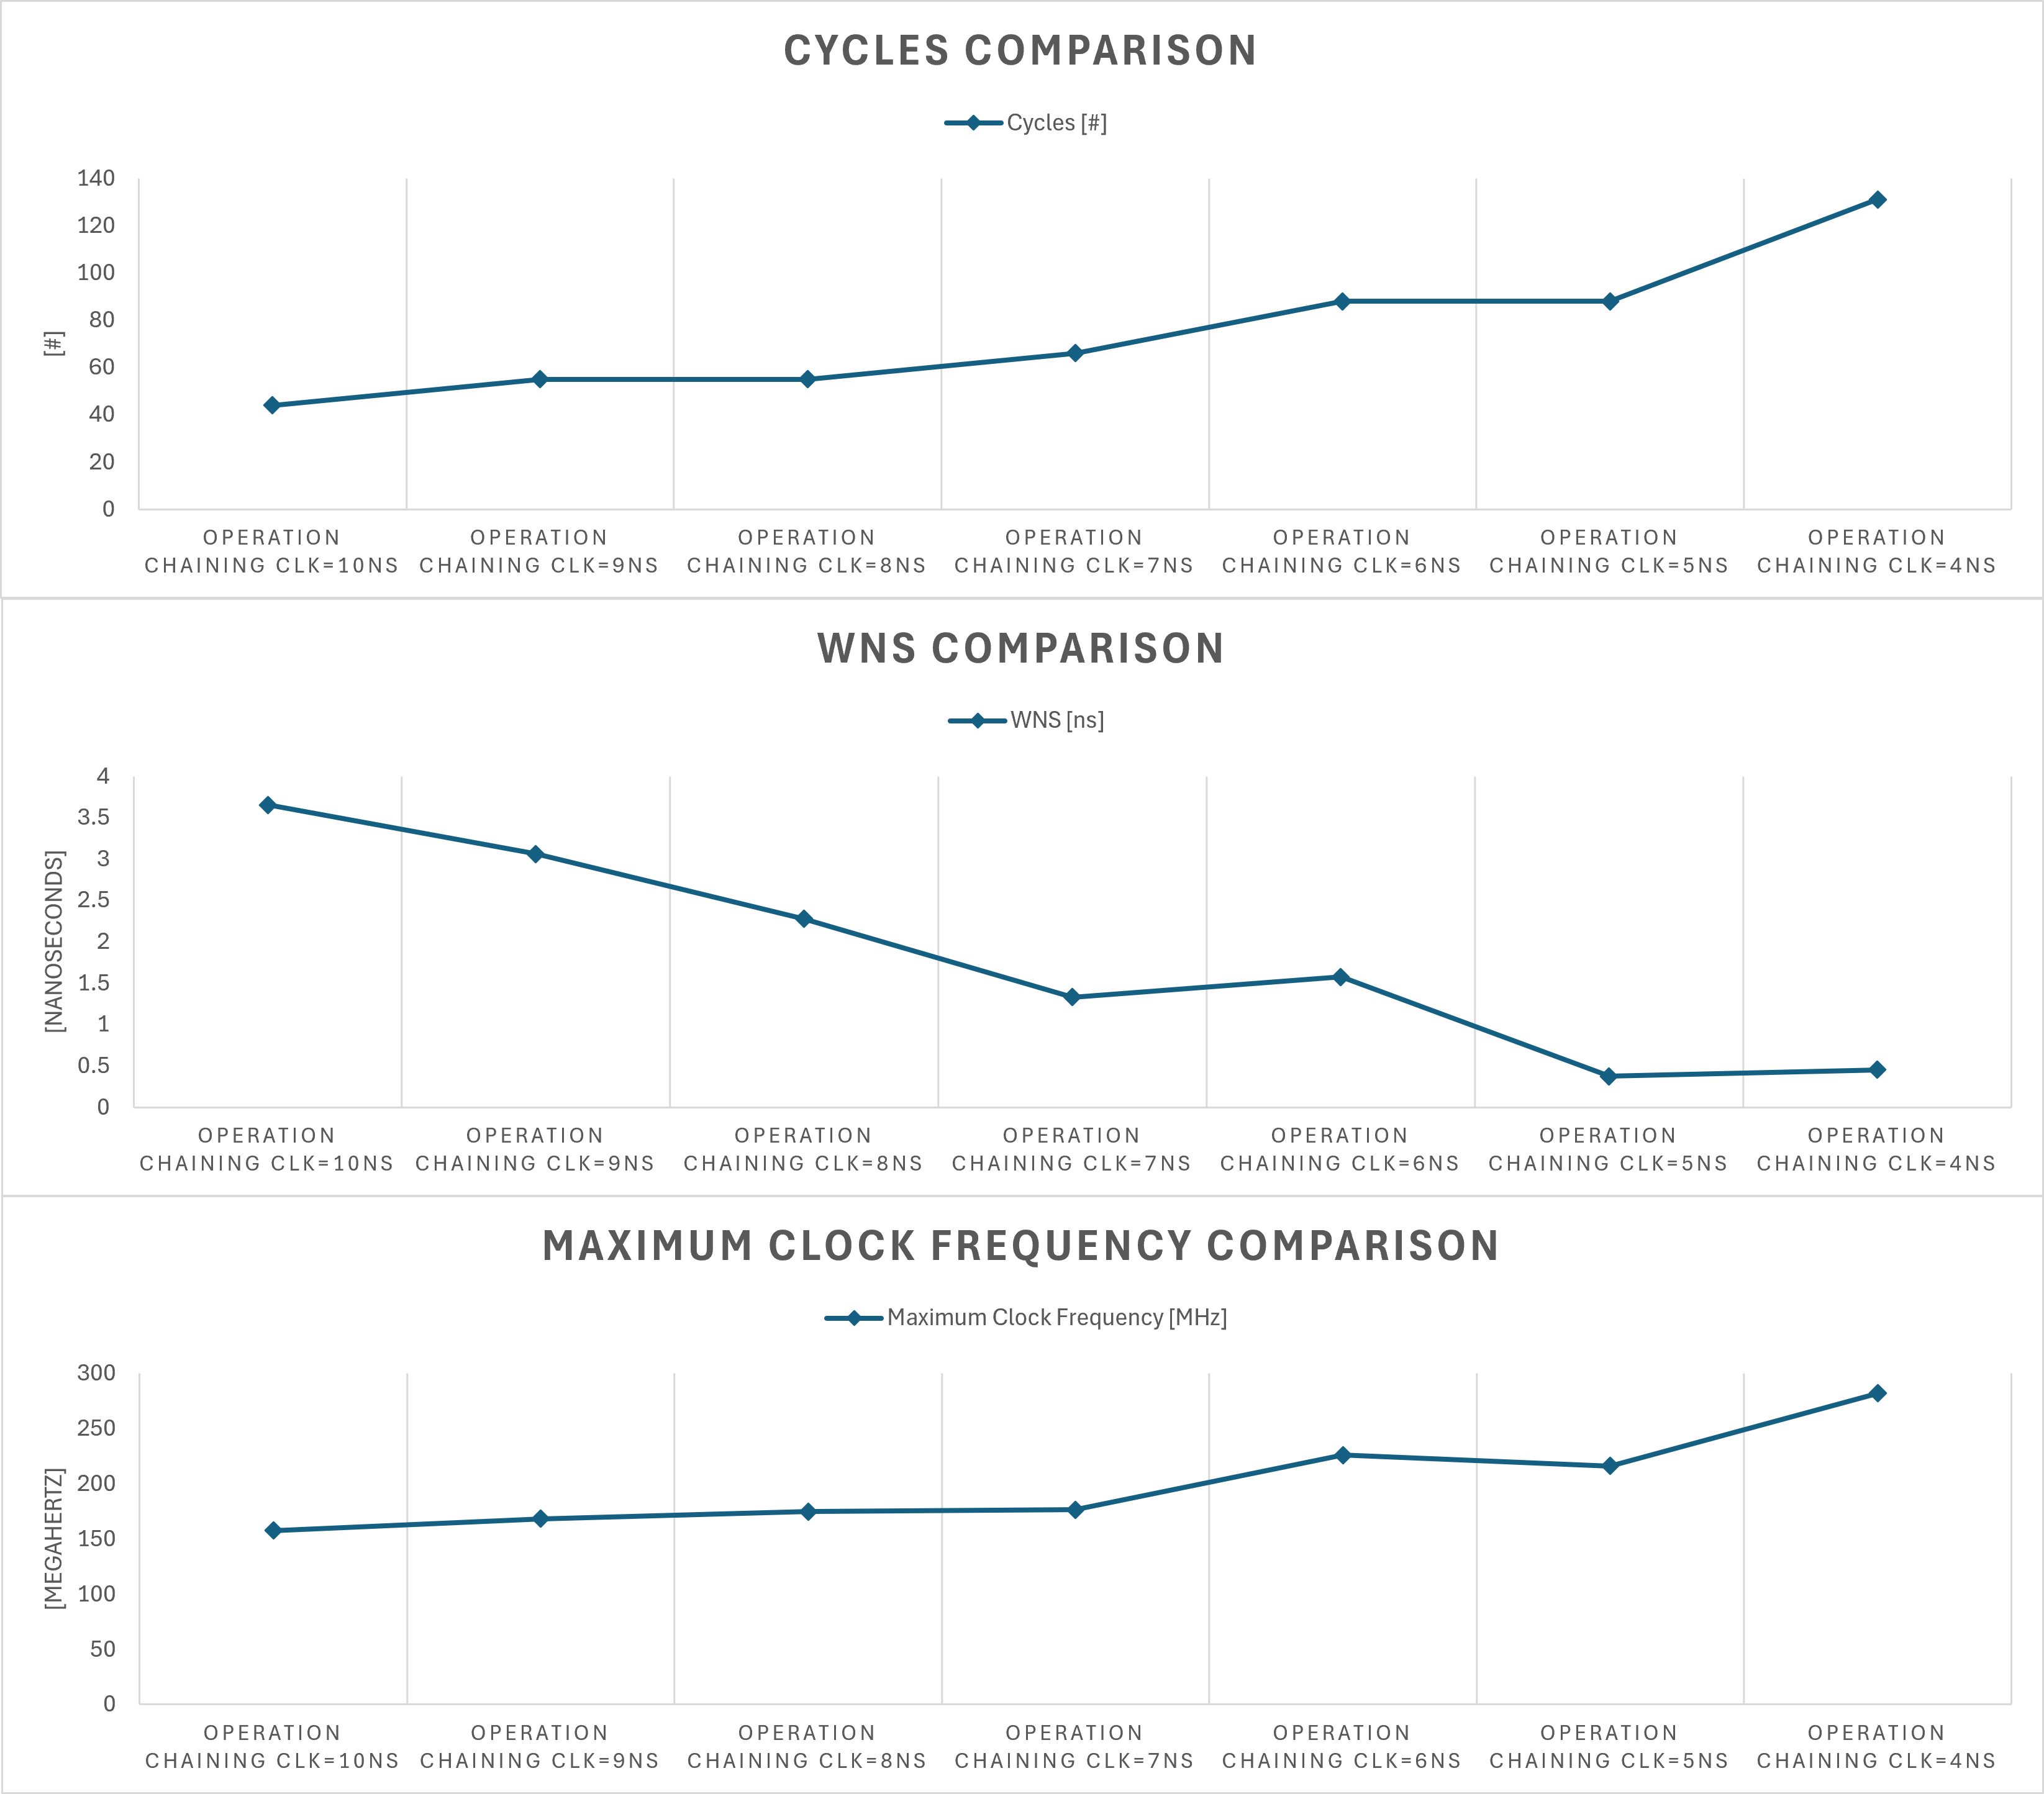
\includegraphics[width=\textwidth]{solutions/operation_chaining/operationchainingtiming.png}
    \caption{Vivado Operation Chaining Timing Plot}
    \label{fig:vivado-operation-chaining-timing-plot}
\end{figure}

Si può notare come in corrispondenza dell'architettura hardware a cui corrisponde un periodo di clock pari a 7ns si ha l'utilizzazione delle risorse minore a meno del numero di LUT e FF che risulta essere aumentato rispettivamente di un'unità e di 66 unità. Questo aumento di risorse può essere giustificato dal momento che, rispetto alla soluzione iniziale non ottimizzata a 10ns, il periodo del clock risulta essere diminuito e, pertanto, il tool prevede una gestione delle istruzioni in maniera più complessa comportando un'aumento delle risorse stesse. Tanto è vero che al diminuire del periodo di clock, si ha un aumento delle risorse utilizzate e dei cicli di clock considerati per ottenere un nuovo risultato. In particolare, per quanto riguarda la massima frequenza di clock associata ad ogni soluzione proposta in questa sezione, si può notare come quella a cui corrisponde un periodo di clock pari a 7ns, presenta una maximum clock frequency maggiore rispetto a quelle avente periodo maggiore. Questo aumento lo si può, inoltre, evidenziare nelle successive soluzioni aventi periodo di clock ancora minore. Tanto è vero che il WNS, al diminuire del clock constraint, anch'esso diminuisce.

\begin{table}[H]
    \centering
    \begin{tabular}{|c|c|c|c|c|c|c|}
        \hline
        \textbf{Solution} & \textbf{Clock Enable} & \textbf{Clocks} & \textbf{DSP} & \textbf{Logic} & \textbf{Set/Reset} & \textbf{Data} \\
        \hline
        clk=10ns & 0.455035944 & 1.215706812 & 0.343570428 & 0.925468281 & 0.00349783 & 1.014495501 \\
        \hline
        clk=9ns & 0.371109403 & 1.601127908 & 0.308091694 & 0.871003722 & 0.003504661 & 0.845550094 \\
        \hline
        clk=8ns & 0.432465255 & 1.790320966 & 0.364705513 & 1.03614782 & 0.003386509 & 1.085355412 \\
        \hline
        clk=7ns & 0.4179838 & 1.991891069 & 0.305155962 & 0.881534419 & 0.002575182 & 0.757947506 \\
        \hline
        clk=6ns & 0.367850007 & 2.092533279 & 0.244985771 & 0.788475969 & 0.00273619 & 0.666663051 \\
        \hline
        clk=5ns & 0.556948828 & 3.174162703 & 0.291668839 & 0.943421735 & 0.004532358 & 0.906153 \\
        \hline
        clk=4ns & 0.57213963 & 3.804846667 & 0.253423554 & 0.799402245 & 0.002476984 & 0.756326073 \\
        \hline
    \end{tabular}
    \caption{Vivado Operation Chaining Solution Dynamic Power Report [mW]}
    \label{tab:vivado-operation-chaining-solution-dynamic-power-reproot}
\end{table}

\begin{table}[H]
    \centering
    \begin{minipage}[t]{0.45\linewidth}
        \centering
        \begin{tabular}{|c|c|}
            \hline
            \textbf{Solution} & \textbf{Dynamic Total} \\
            \hline
            clk=10ns & 3.957774796 \\
            \hline
            clk=9ns & 4.000387481 \\
            \hline
            clk=8ns & 4.712381475 \\
            \hline
            clk=7ns & 4.357087937 \\
            \hline
            clk=6ns & 4.163244267 \\
            \hline
            clk=5ns & 5.876887463 \\
            \hline
            clk=4ns & 6.188615153 \\
            \hline
        \end{tabular}
        \caption{Vivado Operation Chaining Solution Dynamic Power Report [mW]}
        \label{tab:vivado-operation-chaining-solution-dynamic-power-reproot}
    \end{minipage}
    \hfill
    \centering
    \begin{minipage}[t]{0.45\linewidth}
        \centering
        \begin{tabular}{|c|c|}
            \hline
            \textbf{Solution} & \textbf{Energy Single Operation} \\
            \hline
            clk=10ns & 39.57774796 \\
            \hline
            clk=9ns & 36.00348733 \\
            \hline
            clk=8ns & 37.6990518 \\
            \hline
            clk=7ns & 30.49961556 \\
            \hline
            clk=6ns & 24.9794656 \\
            \hline
            clk=5ns & 29.38443731 \\
            \hline
            clk=4ns & 24.75446061 \\
            \hline
        \end{tabular}
        \caption{Vivado Operation Chaining Solution Energy Single Operation Report [pJ]}
        \label{tab:vivado-operation-chaining-solution-solution-energy-single-operation-reproot}
    \end{minipage}
\end{table}

\begin{figure}[H]
    \centering
    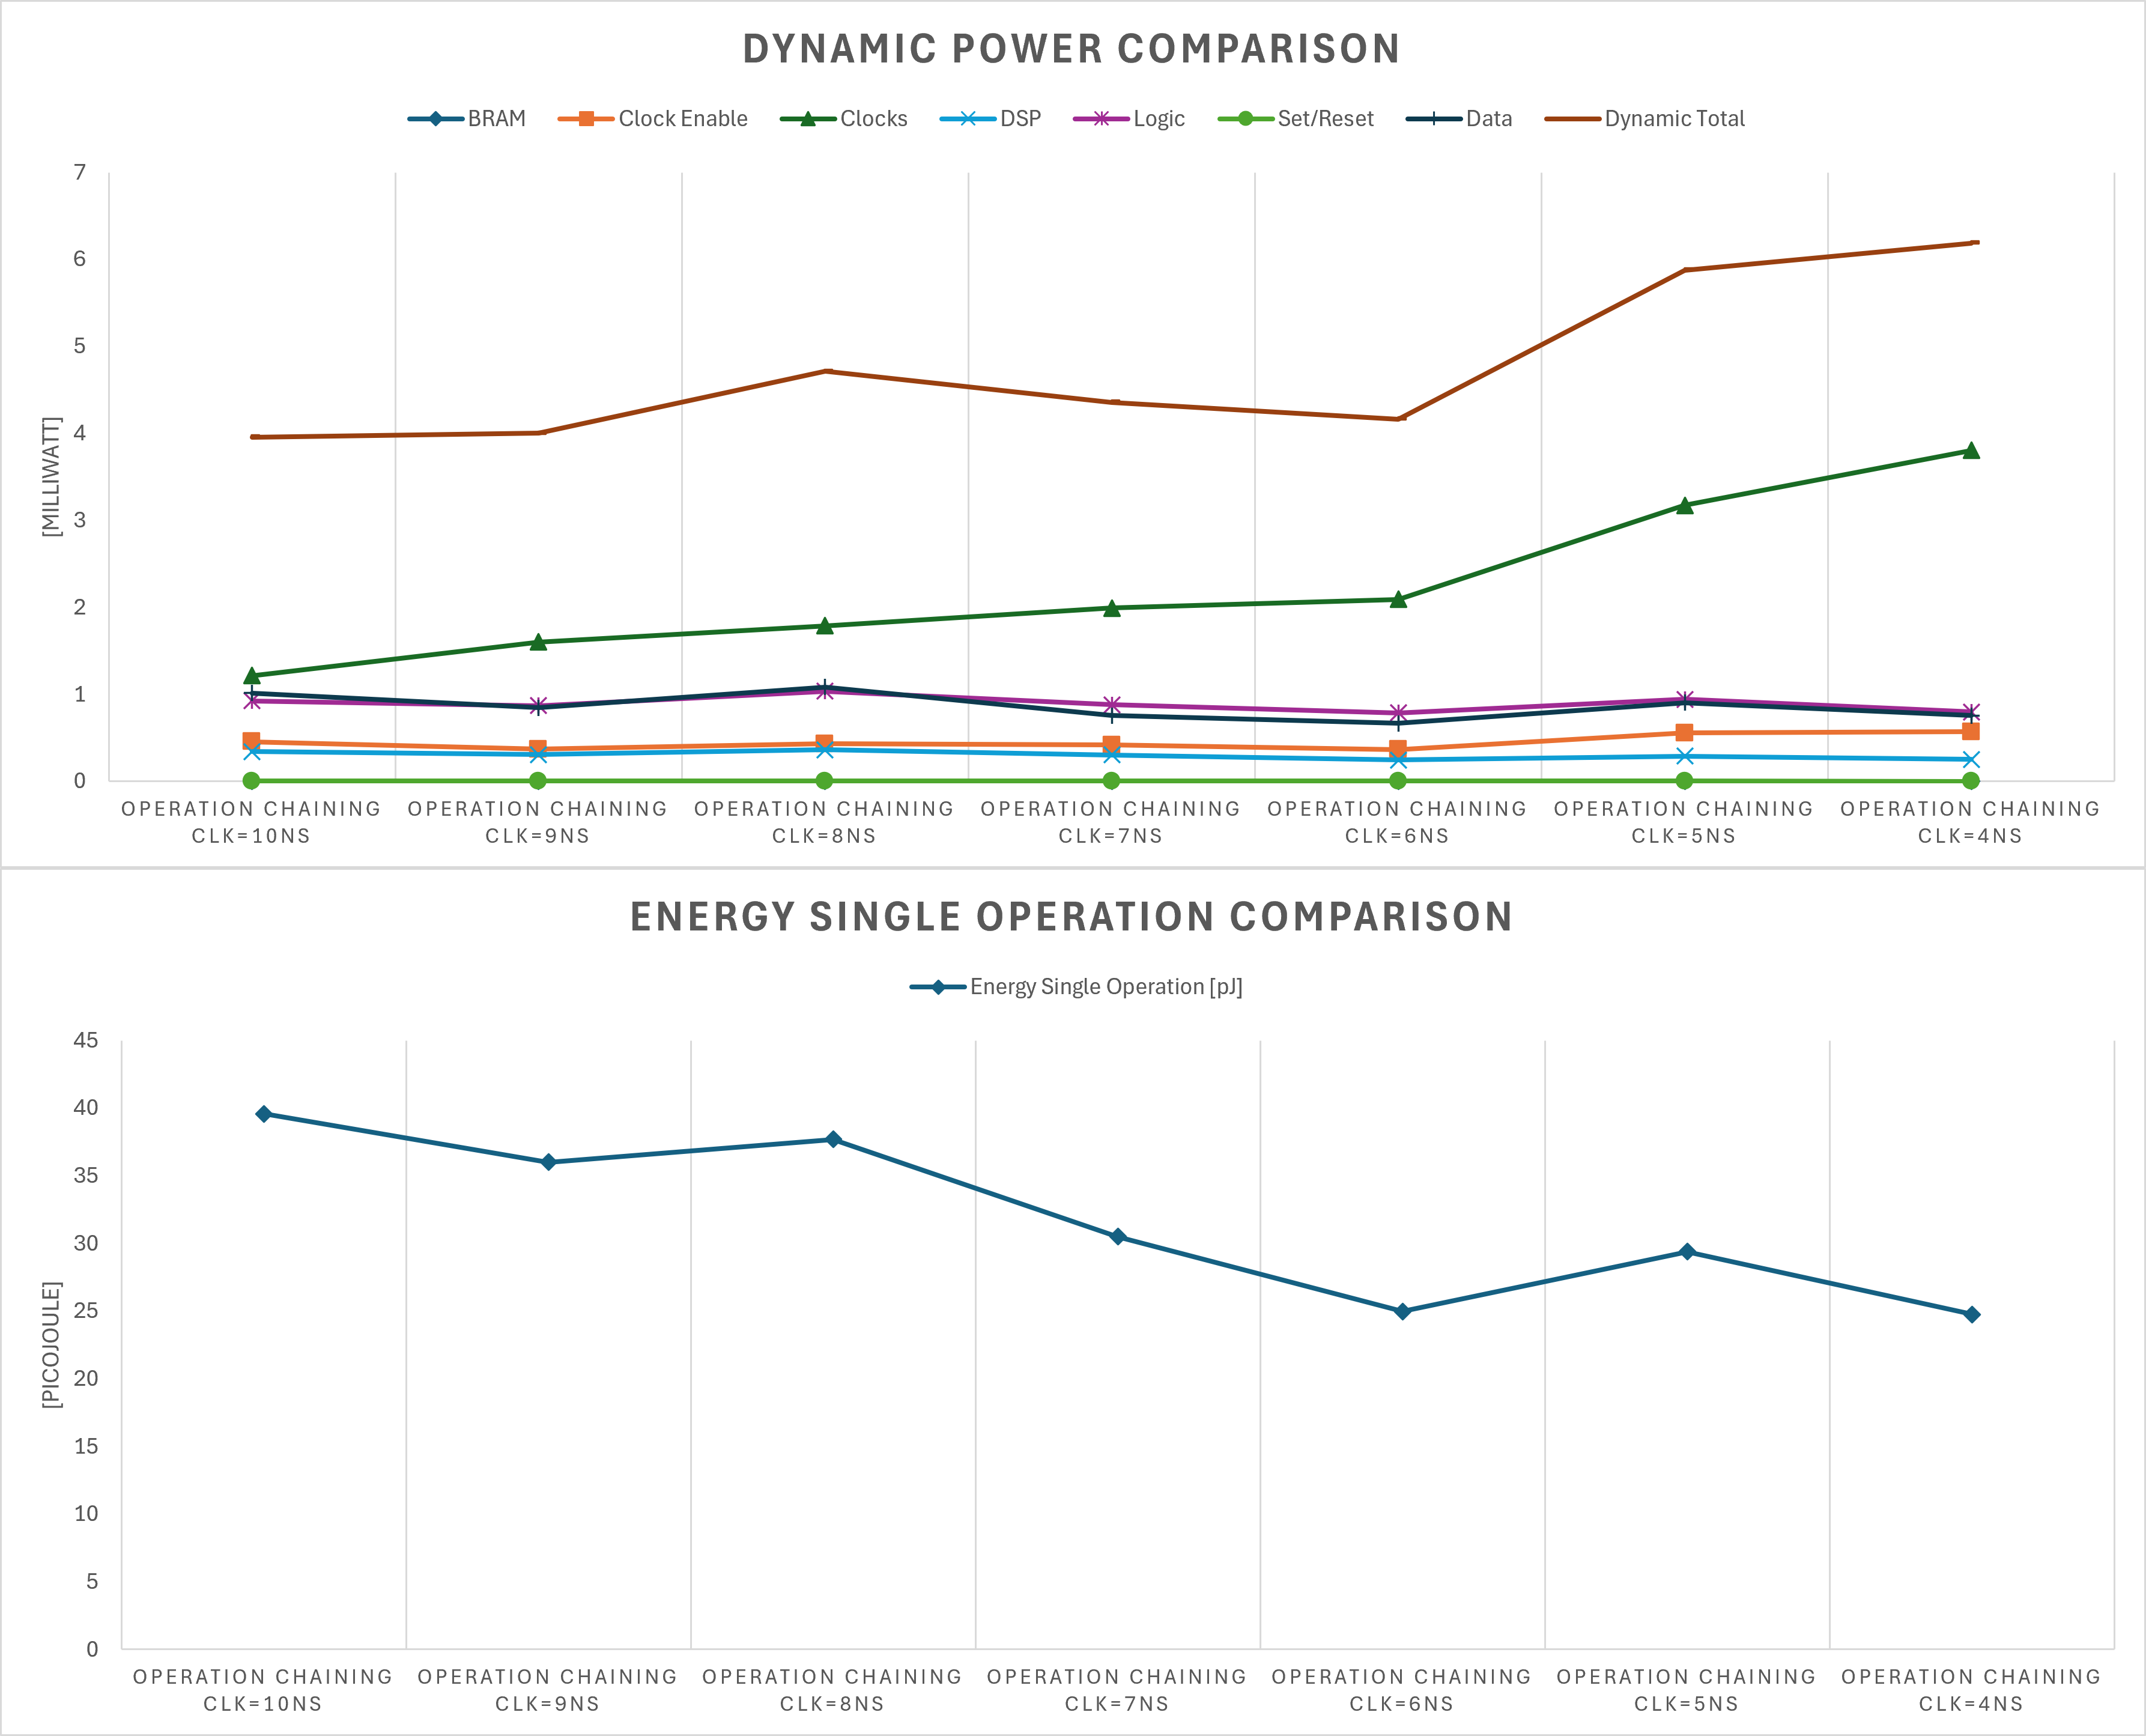
\includegraphics[width=\textwidth]{solutions/operation_chaining/operationchainingpower.png}
    \caption{Vivado Operation Chaining Power Plot}
    \label{fig:vivado-operation-chaining-power-plot}
\end{figure}

Si può notare come la potenza dinamica aumenti al diminuire del periodo di clock considerato. Questo si evince dal fatto che l'utilizzazione delle risorse (in particolar modo per quello che riguarda i FF) aumenta al diminuire del constraint di clock. Tanto è vero che la potenza dinamica associata all'albero di distribuzione del clock (BUFG) e del clock enable sia di gran lunga maggiore rispetto alla soluzione iniziale dove è stato considerato un constraint pari a 10ns. In particolare, questo aumento di potenza dinamica può essere associato al maggior numero di Flip Flop utilizzato nelle soluzioni aventi periodo di clock sempre minore.
\\
Pertanto, considerando i report di utilizzazione delle risorse, di timing, di potenza dinamica ed energia per singola operazione, si può evincere che la soluzione hardware che permette un trade-off ottimale è quella ottenuta in corrispondenza del periodo di clock pari a 7ns.